% How Snooze Oracle works. Needs Inter-Regular.ttf and Inter-SemiBold.ttf (SIL OFL, rsms.me/inter) next to this file.
% Build: tectonic pipeline.tex, then render pipeline.pdf to docs/img/pipeline.png at 300 dpi.
\documentclass[tikz,border=0pt]{standalone}
\usepackage{fontspec}
\setmainfont{Inter-Regular.ttf}[Path=./, BoldFont=Inter-SemiBold.ttf]
\setsansfont{Inter-Regular.ttf}[Path=./, BoldFont=Inter-SemiBold.ttf]
\hyphenpenalty=10000 \exhyphenpenalty=10000 \frenchspacing
\usetikzlibrary{positioning,arrows.meta,calc,backgrounds,fit}
\definecolor{bg}{HTML}{0D1430}
\definecolor{card}{HTML}{1A2246}
\definecolor{line}{HTML}{3A4470}
\definecolor{ink}{HTML}{EEF1FB}
\definecolor{ink2}{HTML}{B6BDD6}
\definecolor{sky}{HTML}{56B4E9}
\definecolor{dawn}{HTML}{F6C96B}
\definecolor{stop}{HTML}{FF8A6A}
\begin{document}
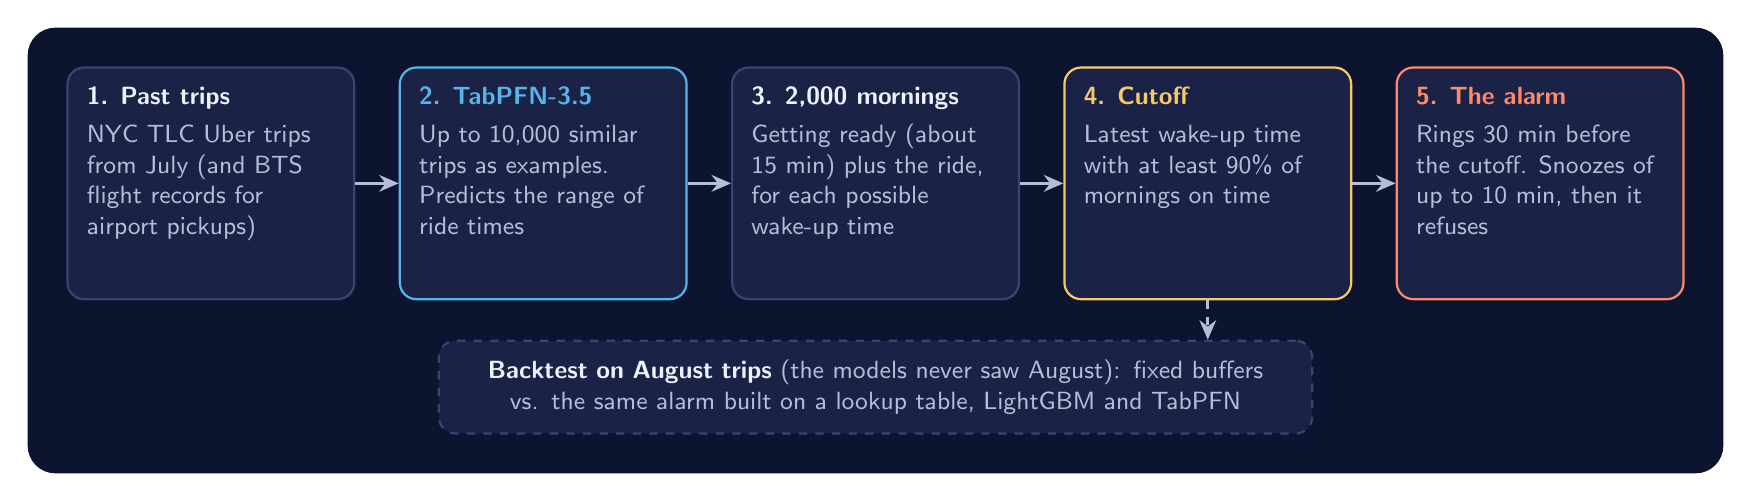
\begin{tikzpicture}[
  font=\sffamily\small, text=ink,
  box/.style={draw=line, line width=0.8pt, fill=card, rounded corners=6pt, align=left,
              inner sep=7pt},
  top/.style={},
  head/.style={font=\bfseries\normalsize},
  arr/.style={-{Stealth[length=7pt,width=6pt]}, line width=1.2pt, draw=ink2},
]
\node[box] (data) {\parbox[t][2.45cm][t]{3.15cm}{\raggedright {\color{ink}\bfseries 1. Past trips}\\[3pt]
  {\color{ink2}NYC TLC Uber trips from July (and BTS flight records for airport pickups)}}};
\node[box, right=0.55cm of data, draw=sky] (tab) {\parbox[t][2.45cm][t]{3.15cm}{\raggedright {\color{sky}\bfseries 2. TabPFN-3.5}\\[3pt]
  {\color{ink2}Up to 10,000 similar trips as examples. Predicts the range of ride times}}};
\node[box, right=0.55cm of tab] (sim) {\parbox[t][2.45cm][t]{3.15cm}{\raggedright {\bfseries 3. 2,000 mornings}\\[3pt]
  {\color{ink2}Getting ready (about 15 min) plus the ride, for each possible wake-up time}}};
\node[box, right=0.55cm of sim, draw=dawn] (wake) {\parbox[t][2.45cm][t]{3.15cm}{\raggedright {\color{dawn}\bfseries 4. Cutoff}\\[3pt]
  {\color{ink2}Latest wake-up time with at least 90\% of mornings on time}}};
\node[box, right=0.55cm of wake, draw=stop] (alarm) {\parbox[t][2.45cm][t]{3.15cm}{\raggedright {\color{stop}\bfseries 5. The alarm}\\[3pt]
  {\color{ink2}Rings 30 min before the cutoff. Snoozes of up to 10 min, then it refuses}}};
\foreach \a/\b in {data/tab, tab/sim, sim/wake, wake/alarm} \draw[arr] (\a) -- (\b);
\node[below=0.5cm of $(tab.south)!0.5!(wake.south)$, draw=line, dashed, line width=0.8pt, fill=card,
      rounded corners=6pt, inner sep=7pt, text width=10.6cm, align=center]
  (test) {{\bfseries Backtest on August trips} {\color{ink2}(the models never saw August):
  fixed buffers vs. the same alarm built on a lookup table, LightGBM and TabPFN}};
\draw[arr, dashed] (wake.south) -- (wake.south |- test.north);
\begin{scope}[on background layer]
  \node[fill=bg, rounded corners=10pt, inner sep=14pt, fit=(data)(alarm)(test)] {};
\end{scope}
\end{tikzpicture}
\end{document}
